\documentclass{beamer}

%TODO: already introduce specification language (needed for mounting+cascading)
%TODO: requirement that data structure should not be directly accessible (environp)
%TODO: add outlook for next lecture

% Make nice A4 pages for print:
%\usepackage{pgfpages}
%\pgfpagesuselayout{resize to}[a4paper,border shrink=5mm,landscape]

\beamertemplatenavigationsymbolsempty

\setbeamertemplate{bibliography item}[text]

\usepackage[type={CC},modifier={by-sa},version={4.0}]{doclicense}

\usepackage[utf8]{inputenc}
\usepackage{hyperref}
\usepackage{breakurl}
\usepackage{graphicx}
\usepackage{pgfplots}
\usepackage{pgf}
\usepackage{tikz}
\usetikzlibrary{positioning}
\usetikzlibrary{arrows}
\usetikzlibrary{decorations.markings}
\usetikzlibrary{calc}
\usetikzlibrary{matrix}
\usetikzlibrary{shapes}
\usetikzlibrary{decorations.pathmorphing}
\usetikzlibrary{fit}
\usetikzlibrary{backgrounds}
\usetikzlibrary{plotmarks}
\usepackage{stmaryrd}
\usepackage{listings}
\usepackage{pdflscape}
\usepackage{perpage}
\usepackage{appendixnumberbeamer}

%\usepackage[thmmarks,amsmath,amsthm]{ntheorem} % already included in beamer
\usepackage{thm-restate}

\usepackage[sort&compress,numbers]{natbib}  % to be have \citet, \citeauthor, \citeyear

\MakePerPage{footnote}

\tikzstyle{o}=[r,ppBlue]
\tikzstyle{r}=[thick,rectangle,align=center]
\tikzstyle{t}=[r,ppTrans] %,font=\bfseries]
\tikzstyle{dd}=[densely dashed]
\tikzstyle{n}=[r,ppBlue]
\tikzstyle{p}=[r,ppRed]
\tikzstyle{ppRed}  =[draw=red,  fill=  red!20]
\tikzstyle{ppBlue} =[draw=blue, fill= blue!20]
\tikzstyle{ppGreen}=[draw=green,fill=green!20]
\tikzstyle{ppTrans}=[draw=none, fill=none]

\usetheme{Warsaw}

\useoutertheme[subsection=true]{smoothbars}
%\useoutertheme[subsection=false]{miniframes}

\definecolor{bblue}{HTML}{D7DF01}	% yellow-ish actually, for better black/white printing
\definecolor{rred}{HTML}{C0504D}
\definecolor{ggreen}{HTML}{9BBB59}
\definecolor{ppurple}{HTML}{9F4C7C}
\definecolor{lightgray}{rgb}{0.3,0.3,0.3}
\definecolor{lightergray}{rgb}{0.9,0.9,0.9}
\definecolor{UniBlue}{RGB}{83,121,170}

\DeclareTextFontCommand\textintro{\normalfont\bfseries\itshape} % nice!
\newcommand{\intro}[2][]
{%
	\textintro{#2}%
}
\newcommand{\empha}[2][]
{%
	\emph{#2}%
}

%\theoremstyle{plain}
\newcounter{reqcounter}
\newtheorem{requirement}[reqcounter]{Requirement}

%setbeamercolor{structure}{fg=violet}

\makeatletter
\def\th@task{%
    \normalfont % body font
    \setbeamercolor{block title example}{bg=orange,fg=white}
    \setbeamercolor{block body example}{bg=orange!20,fg=black}
    \def\inserttheoremblockenv{exampleblock}
  }
\makeatother

\theoremstyle{task}
\newtheorem{task}{Task}

\newenvironment{assignment}%
{%\setbeamercolor{background canvas}{bg=violet}%
%\setbeamercolor{structure}{fg=cyan!90!black}%
 \setbeamercolor{frametitle}{bg=orange,fg=white}
\begin{frame}}%
{\end{frame}}%

\AtBeginSection[]{
  \begin{frame}
  \vfill
  \centering
  \begin{beamercolorbox}[sep=8pt,center,shadow=true,rounded=true]{title}
    \usebeamerfont{title}\insertsectionhead\par%
  \end{beamercolorbox}
  \tableofcontents
  \vfill
  \end{frame}
}




\pgfplotsset{compat=1.14}
\author{Markus Raab}


\date{9.3.2018}

\begin{document}

\renewcommand{\enquote}[1]{\emph{``#1''}} % Cannot be done earlier

%%%%%%%%%%%%%%%%%%%%%%%%%%%%%%%
\begin{frame}
	\titlepage
	\doclicenseThis
\end{frame}

\begin{assignment}
	\frametitle{Language of the Talk?}
	\begin{task}
	Hands up if you prefer German.
	\end{task}
	Unanimous preference of German required, otherwise English.
\end{assignment}

\begin{frame}
	\frametitle{Organization}
	Slides now available at
	\url{https://www.libelektra.org/ftp/elektra/slides/cm/}
	\\[1cm]
	Next lectures:
	\begin{description}
		\item[9.3.2018:] \textbf{TISS registration}
		\item[16.3.2018:] \textbf{topic homework and talk} (GitHub account!)
		\item[23.3.2018:] teams found together
		\item[13.4.2018:] homework submitted, topics of team exercise
		\item[20.4.2018:] \textbf{no lecture}

		\item[18.5.2018:] guest lecture
		\item[25.5.2018:] team exercise submitted
		\item[22.6.2018:] last corrections of team exercise
		%\item[29.6.2018:] test
	\end{description}
\end{frame}


\begin{frame}
	\frametitle{Popular Topics}
	\vspace{-0.5cm}
	\begin{multicols}{2}
	\begin{description}
	\item[4] validation
	\item[4] user interface
	\item[3] tools (benefits?)
	\item[3] testability
	\item[3] complexity reduction (when conf. needed?)
	\item[3] architectural decisions
	\item[2] Puppet
	\item[2] modularity
	\item[2] environment variables
	\item[2] documentation
	\item[2] configuration specification
	\item[2] command-line args
	\item[2] code generation
	\item[1] variability
	\item[1] self-description
	\item[1] round-tripping
	\item[1] introspection
	\item[1] early
	\item[1] dependencies
	\item[1] context-awareness
	\item[1] auto-detection
	\item[1] administrators
	\end{description}
	\end{multicols}
\end{frame}

\begin{frame}
	\hspace*{-1cm}\includegraphics[width=\paperwidth]{dot/topics}
\end{frame}



\section{Configuration File Formats}

\subsection{Definitions}

\begin{frame}
	\frametitle{Basic Definitions}
	The \intro[execution environment]{execution environment} is information outside the boundaries of each currently running process~\cite{corbato1971multics}.

	Controlling the execution environment is essential for configuration management~\cite{cons2002pan,huang2015confvalley}, testing~\cite{van2010automating,wang2009context}, and security~\cite{goldberg1996secure,schreuders2012towards,perkins2009automatically,liang2003isolated}.
\end{frame}

\begin{frame}
	\frametitle{Configuration Setting}
	\begin{definition}
\label{def:configuration-setting}
A \intro[configuration setting]{configuration setting},
or \intro[setting|see{configuration setting}]{setting} in short,
fulfills these properties:
\begin{enumerate}
\item
It is provided by the execution environment.
\item
It is \empha[consume]{consumed} by an application.
\item
It consists of a key, a configuration value, and potentially \empha{metadata}.
The \intro{configuration value}, or \intro[value|see{configuration value}]{value} in short, influences the application's behavior.
\item
It can be \empha[produce]{produced} by the maintainer, user, or system administrator of the software.
\end{enumerate}
\end{definition}

\end{frame}


\begin{frame}[fragile]
	\frametitle{Synonyms for Configuration Settings}
	\ExecuteMetaData[../book/background.tex]{synonyms}
\end{frame}

\begin{frame}[fragile]
	\frametitle{Definition}
	A \intro{configuration file} is a file containing configuration settings.

	\pause
	A Web server configuration file:

	\begin{lstlisting}[gobble=4]
	port=80 ; comment
	address=127.0.0.1\end{lstlisting}

	\only<2-2>{
	\begin{task}
	What are keys? What are configuration values? What is metadata?
	\end{task}
	}
	\pause

	The configuration values are ^80^ and ^127.0.0.1^, respectively.
	Other information in the configuration file is metadata for the configuration settings (such as the comment).
\end{frame}

\subsection{Formats}

\begin{frame}
	\frametitle{Types of Formats}
	\begin{itemize}
	\item CSV (comma-separated values)
	\item semi-structured
	\item programming language
	\item document-oriented, literate
	\item especially made (easy to use vs.\ easy to implement)
	\end{itemize}
\end{frame}

\begin{frame}
	\frametitle{CSV formats}
	\begin{itemize}
	\item passwd: \formatdate{3}{11}{1971}
	\item passwd and group use : as separator
	\item are difficult to extend (e.g., GECOS)
	\item only used for legacy reasons
	\item are replaced one-by-one (e.g., inetd, crontab)
	\end{itemize}
\end{frame}

\begin{frame}
	\frametitle{Trends}
	\begin{itemize}
	\item away from CSV
	\item towards general-purpose serialization formats (INI, JSON)
	\item human-read/writable (YAML, HOCON, TOML)
	\item programming language as configuration file
	\end{itemize}
\end{frame}

\begin{assignment}
	\frametitle{Introduce somebody}
	\begin{task}
	Talk with someone else about your favourite configuration file format.
	\end{task}

	\begin{task}
	Did you implement a configuration file parser and/or invented a new configuration file format?
	\end{task}

	\begin{task}
	Explain to everyone about the other person and his/her favourite configuration file format.
	\end{task}
\end{assignment}

\begin{frame}
	\frametitle{Method}
	\begin{description}
	\item[\methodSource{}] source code analysis of 16 applications, comprising 50 million lines of code~\cite{raab2017challenges}
	\item[\methodQuestion{}] survey with 672 persons visiting, 162 persons completing the survey~\cite{raab2017challenges}
	\end{description}
\end{frame}

\begin{frame}
	\frametitle{Why are so many formats present?}
	\methodQuestion{} \question{In which way have you used or contributed to the configuration system/library/API in your previously mentioned FLOSS project(s)?}~\cite{raab2017challenges}
	\begin{itemize}
	\item \p{19} persons ($n=251$) claim to have introduced a configuration file format.
	\item \p{29} implemented a configuration file parser.
	\item \p{15} introduced a configuration system/library/API.
	\item used external configuration access APIs (\p{34}).
	\end{itemize}
\end{frame}



\subsection{Abstractions}

\begin{frame}
	\frametitle{Abstraction}
	\begin{restatable}{requirement}{reqLegacy}
	A configuration library must be able to integrate (legacy) systems and must fully support (legacy) configuration files.%
	\label{req:legacy}
	\end{restatable}

	\vspace{1cm}

	How can we deal with the many formats?
\end{frame}


\begin{frame}
	\frametitle{Key-Value}
A key-value pair is the simplest generic data structure~\cite{strang2004context}.
While all these formats above have many differences, all of them represent configuration settings as \intro[key-value pair]{key-value pairs}~\cite{jin2014configurations,rabkin2011static,xu2013blame,lathia2013open}.
\\[1cm]

For configuration as program you need to execute them first.
\end{frame}

\begin{frame}
	\frametitle{Mounting}
	\intro[mounting]{Mounting} integrates a backend into the key database~\cite{raab2008thesis}.
	Hence, \elektra{} allows several backends to deal with configuration files at the same time.
	Each backend is responsible for its own subtree of the key database.

	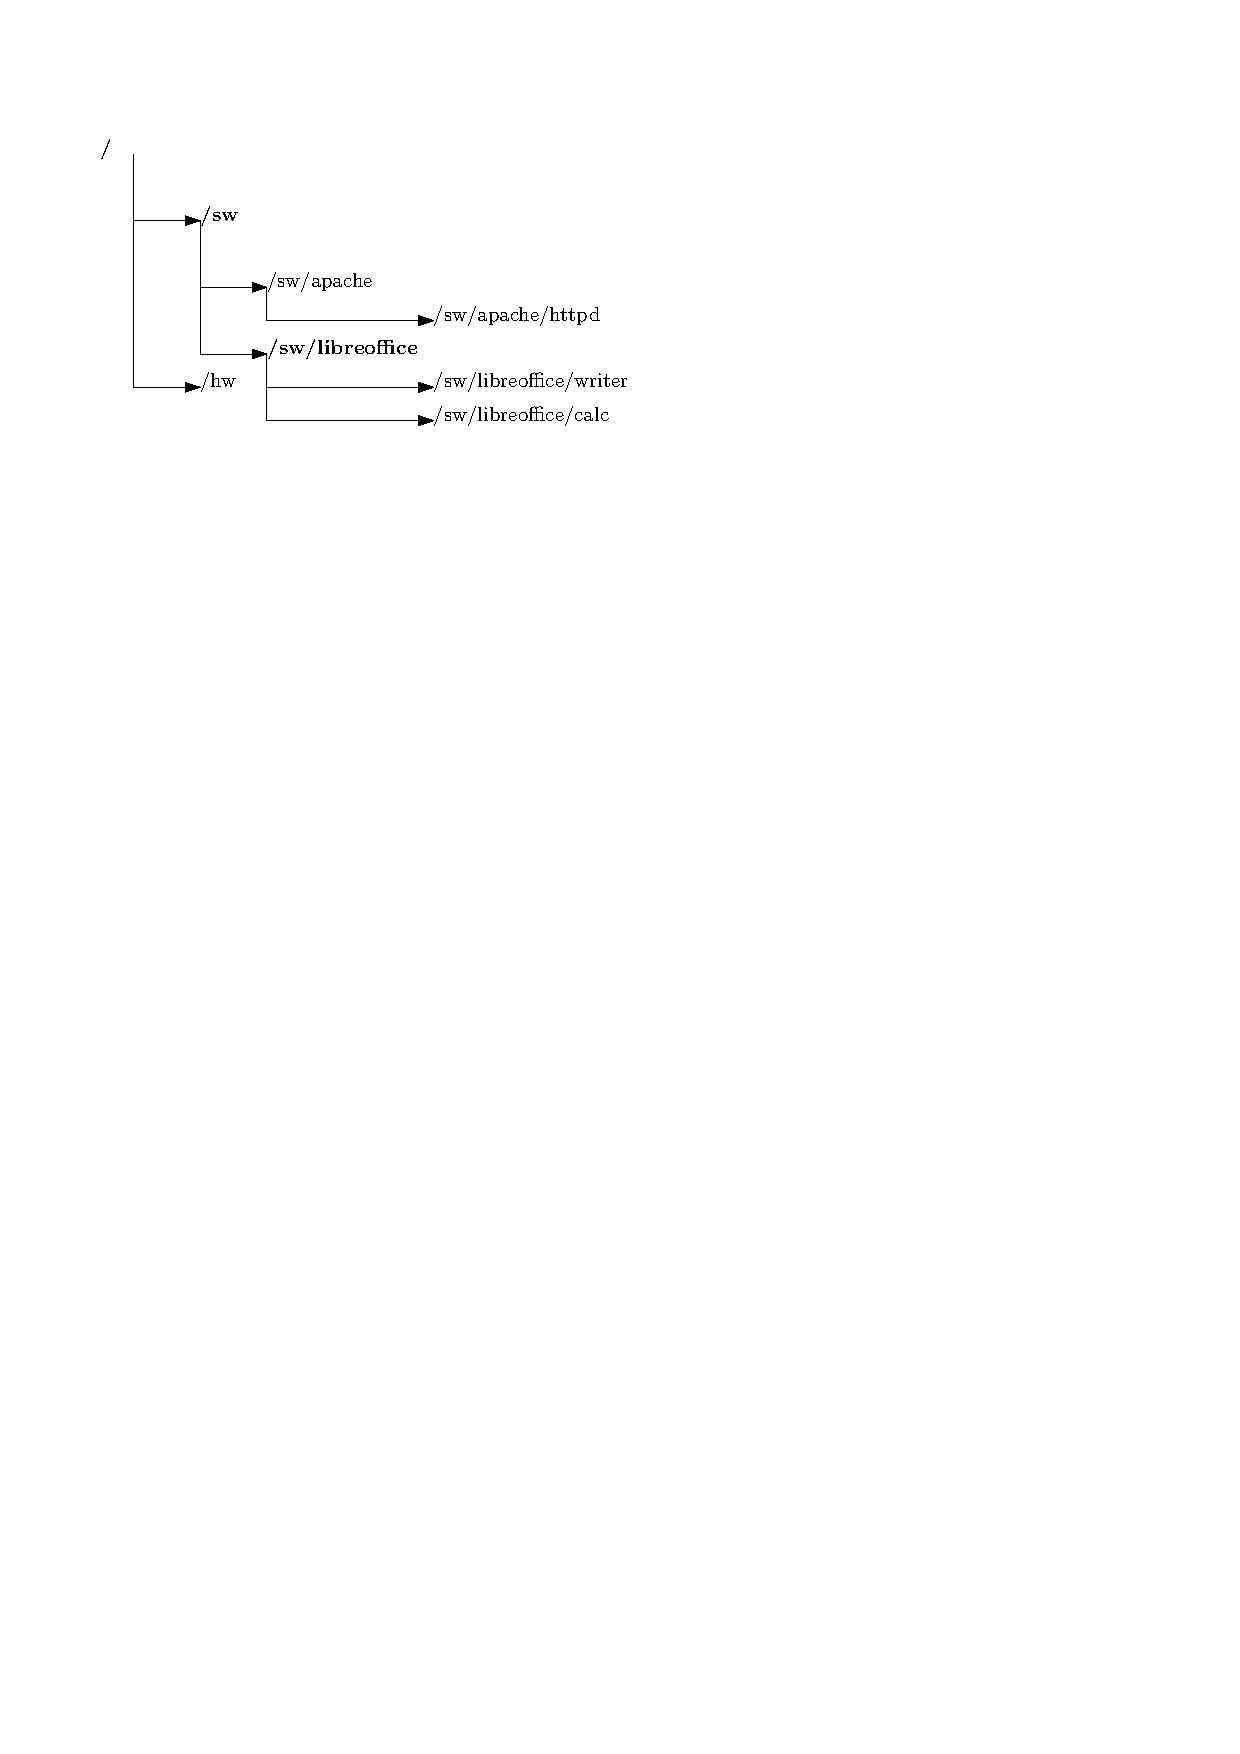
\includegraphics{mounting}
\end{frame}

\begin{frame}
	\frametitle{Plugins}

	Different backends can use different plugins:
	\begin{description}[labelsep=10cm,align=right]
	\item[\texttt{/sw}] in the INI file config.ini
	\item[\texttt{/sw/libreoffice}] in the XML file libreoffice.xml
	\end{description}

	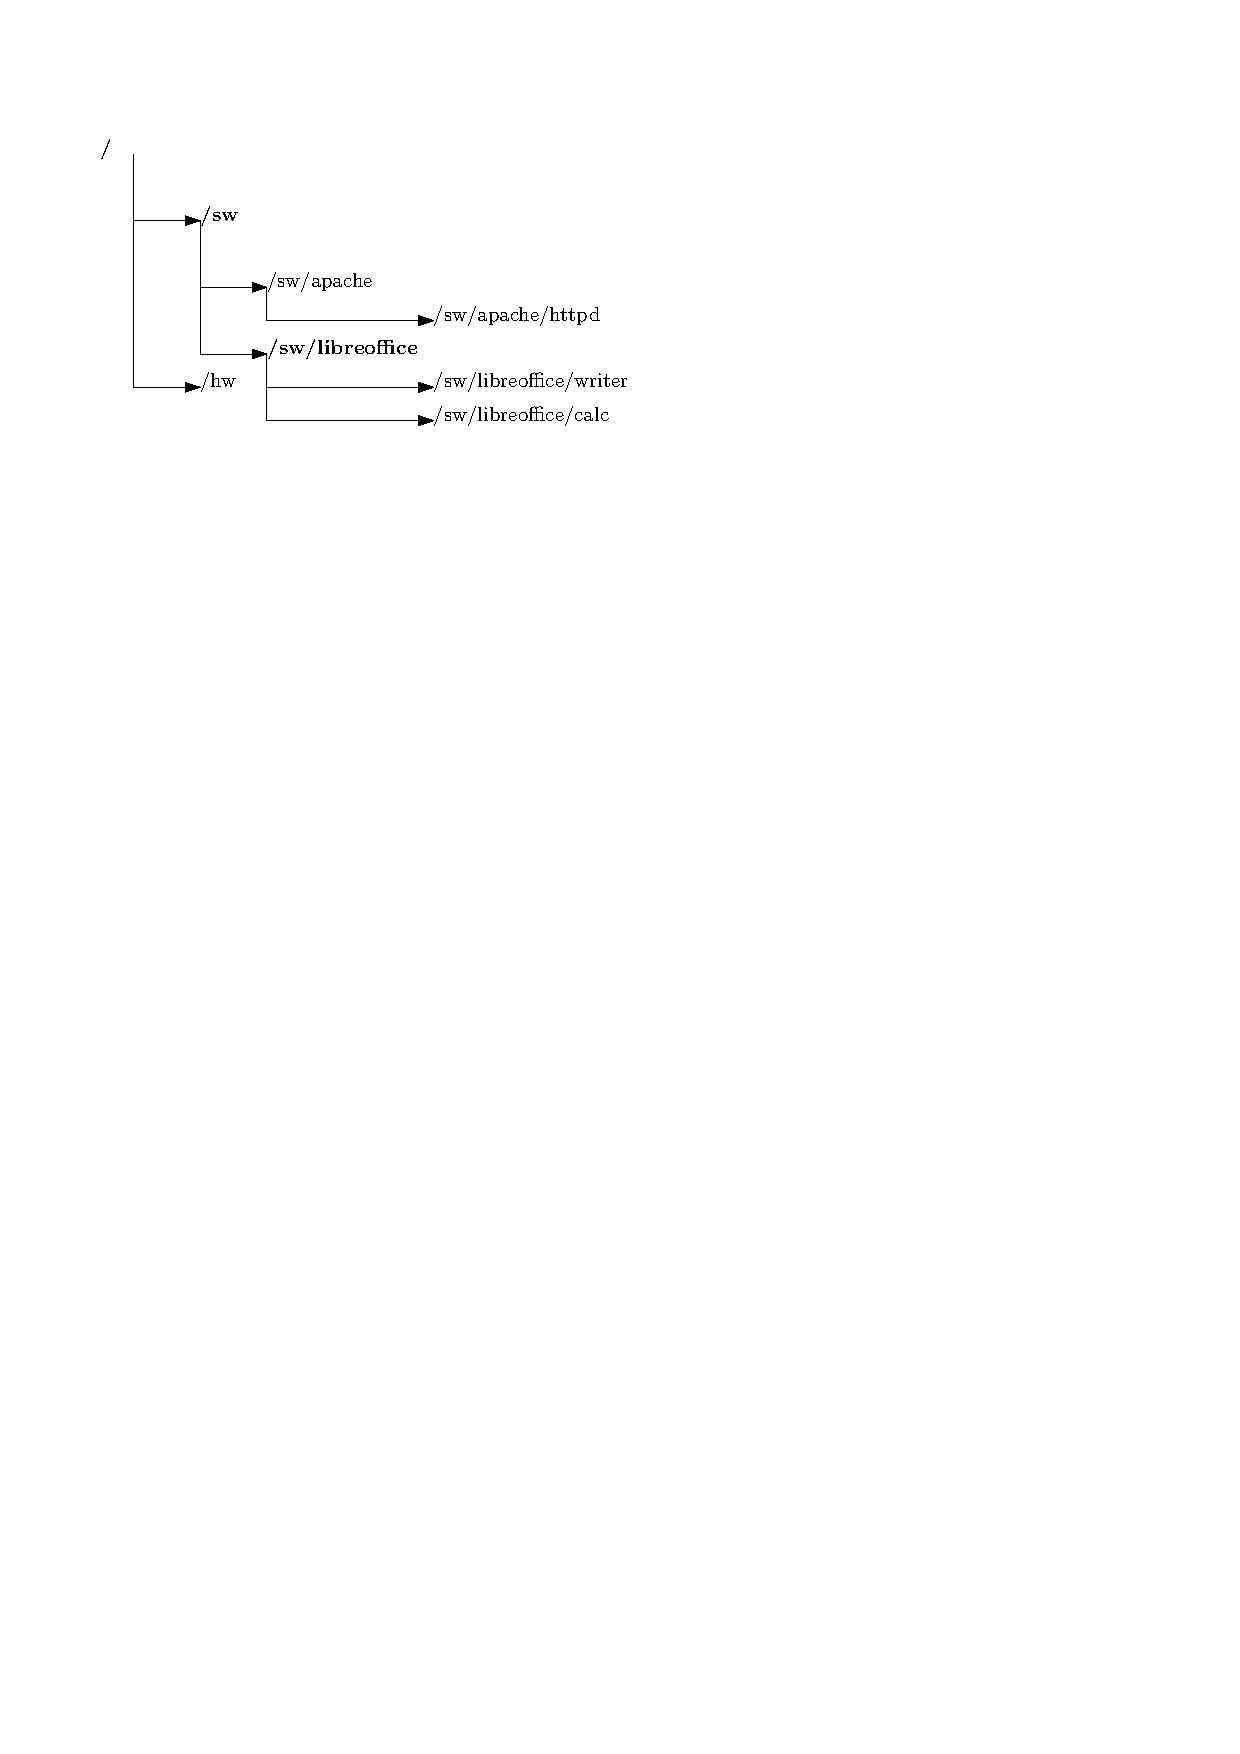
\includegraphics{mounting}
\end{frame}

\begin{assignment}
	\begin{task}
	Possible Homework: Implement a storage plugin with existing parser.
	\end{task}

	\begin{task}
	Explain your neighbor what mounting is.
	\end{task}
\end{assignment}


%%%%%%%%%%%%%%%%%%%%%%%%%%%%%%%%%%%%%%%%%% 
\section{Command-line Arguments}

\subsection{Usage and Popularity}

\begin{frame}
	\frametitle{Is there something else?}
	\begin{itemize}
	\item configuration files are the most researched of all configuration sources~\cite{jin2014configurations}
	\item but it is neither the most used nor most popular~\cite{raab2017challenges}
	\end{itemize}
\end{frame}

\begin{frame}
	\methodQuestion{} \question{Which configuration systems/libraries/APIs have you already used or would like to use in one of your FLOSS project(s)?}
	\begin{itemize}
	\item command-line arguments (\p{92}, $n=222$)
	\item environment variables (\p{79}, $n=218$)
	\item \methodSource{} API \texttt{getenv} is used omnipresently with 2,683 occurrences
	\item configuration files (\p{74}, $n=218$))
	\end{itemize}
\end{frame}


\begin{frame}
	\methodQuestion{} \question{What is your experience with the following configuration systems/libraries/APIs?}
	\begin{itemize}
	\item \texttt{getenv} (\p{10}, $n=198$)
	\item configuration files (\p{6}, $n=190$)
	\item command-line options (\p{4}, $n=210$)
	\item X/Q/GSettings (\p{41}, \p{14}, \p{35})
	\item KConfig (\p{21})
	\item dconf (\p{42})
	\item plist (\p{32})
	\item Windows Registry (\p{69})
	\end{itemize}
\end{frame}

\begin{assignment}
	\begin{task}
	Which configuration source do you use most?
	\end{task}

	\begin{task}
	Possible talk: About one of these sources.
	\end{task}
\end{assignment}

\subsection{Semantics}

\begin{frame}
	\begin{itemize}
	\item passed by main for a new process via \\ (\texttt{int argc, char ** argv})
	\item visible from other processes (e.g., via \texttt{ps aux})
	\item could be passed along to subprocesses but hardly done
	\item need to be parsed by process
	\item portability: differences in parsing
	\item cannot be changed from outside (requires restart, no IPC)
	\end{itemize}
\end{frame}

%%%%%%%%%%%%%%%%%%%%%%%%%%%%%%%%%%%%%%%%%% 
\section{Environment Variables}

\begin{frame}
	\frametitle{Semantics}
	\begin{itemize}
	\item are also per-process (\texttt{/proc/self/environ})
	\item are not visible from other processes
	\item are automatically inherited by subprocesses
	\item need to be parsed by process (\texttt{[extern] char **environ}) but API is provided (\texttt{getenv})
	\item cannot be changed from outside (requires restart, no IPC)
	\end{itemize}
\end{frame}

\begin{assignment}
	\begin{task}
	What is wrong with the code in the book?
	\end{task}
\end{assignment}

\begin{frame}
	\frametitle{getenv}
	\begin{itemize}
	\item is widely standardized, including SVr4, POSIX.1-2001, 4.3BSD, C89, C99~\cite{man2017getenv},
	\item is supported by many programming languages, and
	\item enforces \texttt{key=value} convention.
	\end{itemize}
\end{frame}

\begin{frame}
	\frametitle{Usage}
	\begin{enumerate}
	\item bypassing other configuration accesses (\methodQuestion{} \p{45})
	\item locating configuration files
	\item debugging and testing (\methodQuestion{} \p{55}, \methodSource{} 1,152, i.\,e. \p{43})
	\item sharing configuration settings across applications (\methodQuestion{} \p{53}, \methodSource{} 716, i.\,e. \p{47})
	\item for configuration settings unlikely to be changed by a user (\methodQuestion{} \p{20})
	\item \question{even when it is used inside a loop} (\methodQuestion{} \p{2})
	\end{enumerate}
\end{frame}

\begin{frame}
	\frametitle{Portability}
	\begin{itemize}
	\item no separators for values defined
	\item case sensitivity problems
	\item often many environment variables for the same purpose: TMP, TEMP, or TMPDIR
	\item sometimes one environment variable for different purposes: PATH
	\end{itemize}
\end{frame}

\subsection{Trends}

\begin{frame}
	\frametitle{Trend Firefox}
	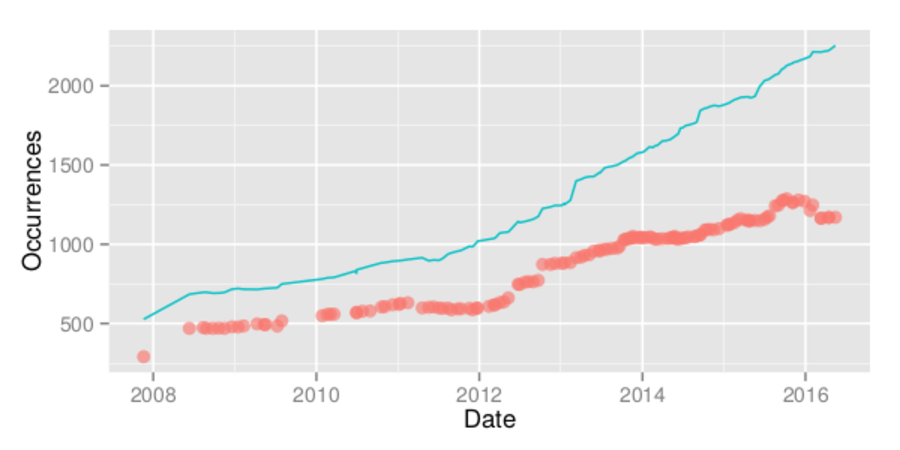
\includegraphics[scale=0.7]{firefox}
\end{frame}

\begin{frame}
	\frametitle{Trend Chromium}
	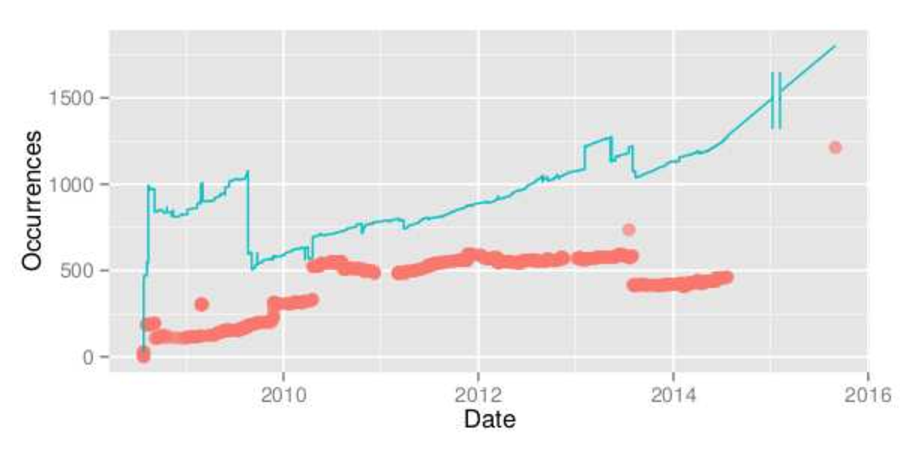
\includegraphics[scale=0.7]{chromium}
\end{frame}

\subsection{Requirements}

\begin{frame}
	How can we deal with the many sources?

	\vspace{1cm}

	\begin{restatable}{requirement}{reqEnvironment}
	A configuration library must support all three popular ways for configuration access:
	configuration files, command-line options, and environment variables.
	\end{restatable}
\end{frame}

\begin{frame}
	\frametitle{Cascading}
	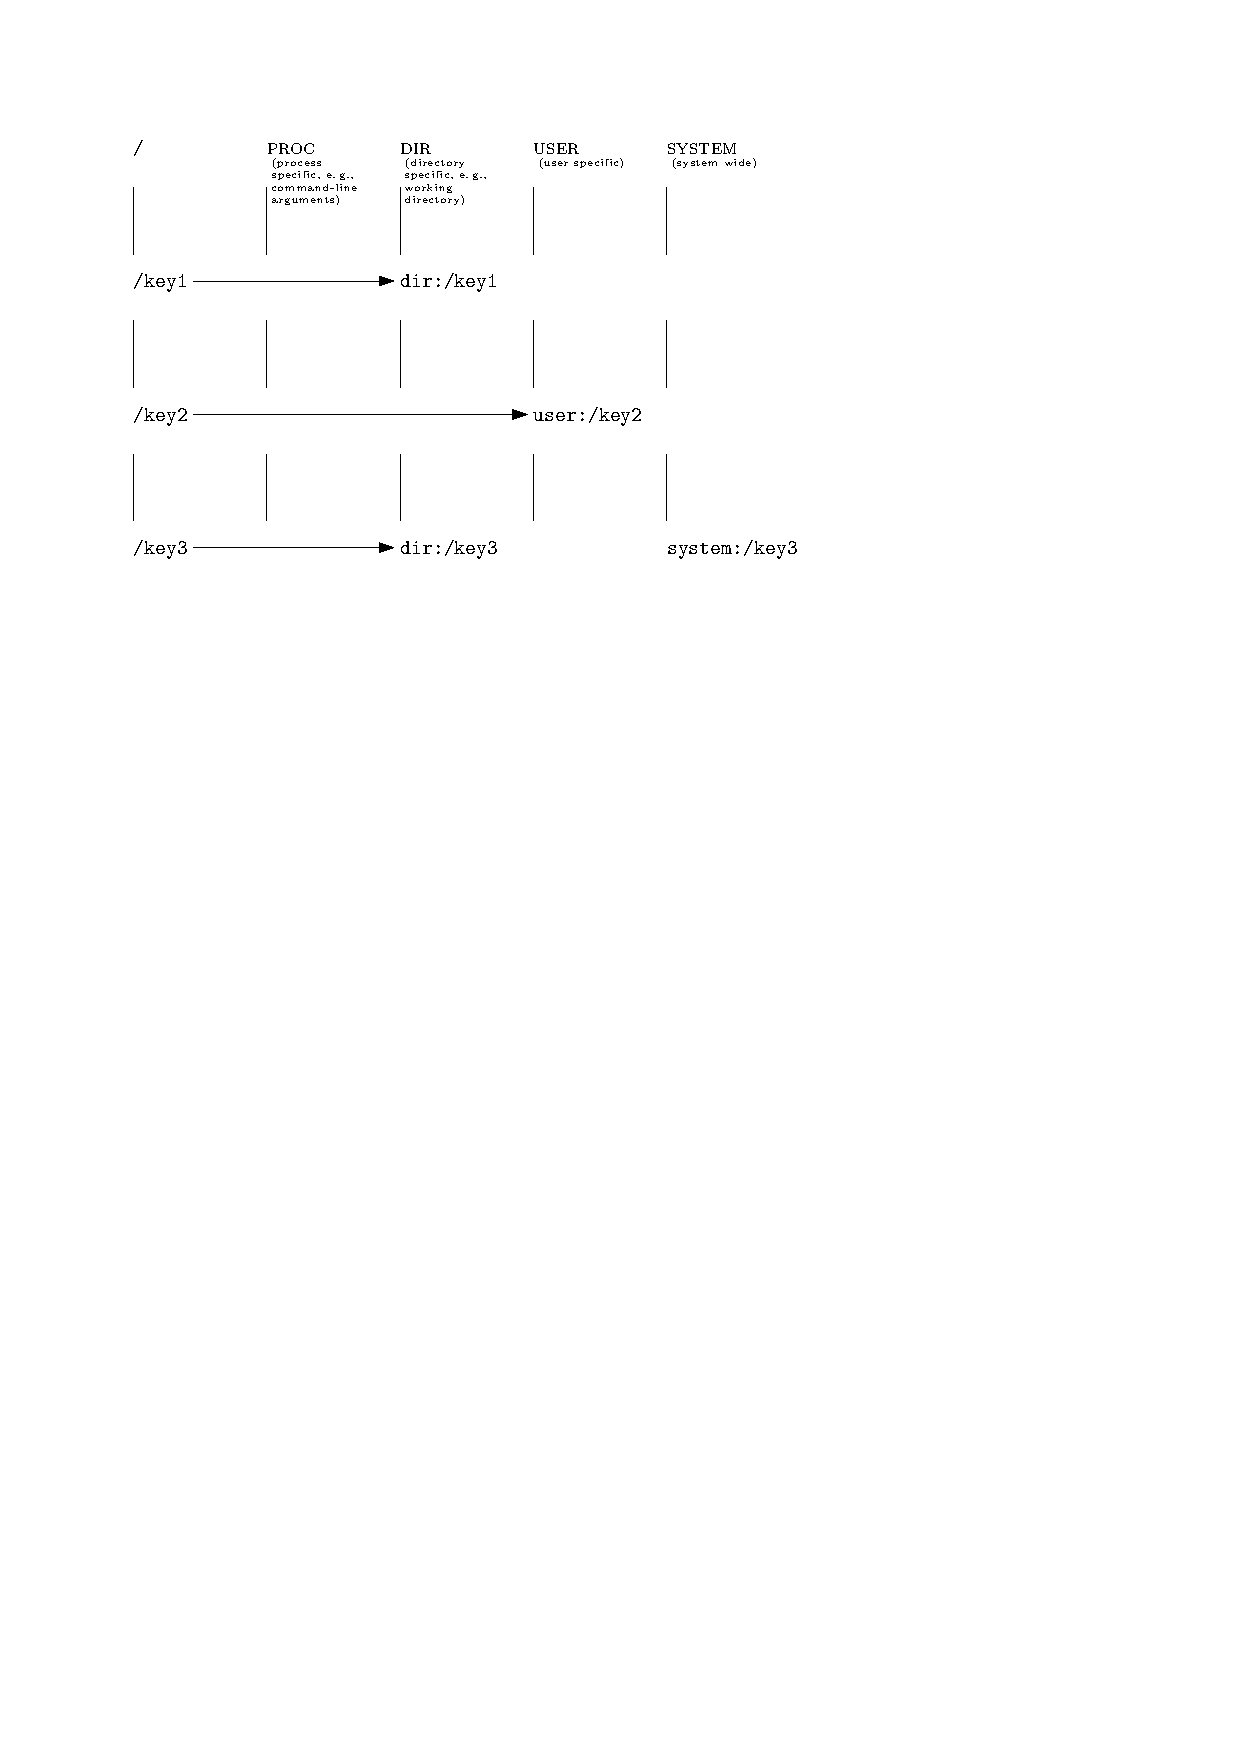
\includegraphics{cascading}
\end{frame}

\begin{assignment}
	\begin{task}
	Discuss the differences of mounting and cascading with your neighbor.
	\end{task}
\end{assignment}

\subsection{Conclusion}

\begin{frame}
	\frametitle{User View}
	\begin{itemize}
	\item command-line for trying out configuration settings
	\item environment variables for configuration settings within a shell
	\item configuration files for persistent configuration settings
	\end{itemize}
\end{frame}

\begin{frame}
	\frametitle{Conclusion}
	\begin{itemize}
	\item three different configuration sources widely used
	\item all three used for different reasons but often for the same configuration settings
	\item many different configuration file formats
	\item abstractions: key-value, mounting, and cascading
	\end{itemize}
\end{frame}



%%%%%%%%%%%%%%%%%%%%%%%%%%%%%%%%%%%%%%%%%% 
\nocite{raab2017introducing}

\appendix

\begin{frame}[allowframebreaks]
	\bibliographystyle{plainnat}
	\bibliography{../shared/elektra.bib}
\end{frame}

\end{document}


